%% ****** Start of file apstemplate.tex ****** %
%%
%%
%%   This file is part of the APS files in the REVTeX 4 distribution.
%%   Version 4.1r of REVTeX, August 2010
%%
%%
%%   Copyright (c) 2001, 2009, 2010 The American Physical Society.
%%
%%   See the REVTeX 4 README file for restrictions and more information.
%%
%
% This is a template for producing manuscripts for use with REVTEX 4.0
% Copy this file to another name and then work on that file.
% That way, you always have this original template file to use.
%
% Group addresses by affiliation; use superscriptaddress for long
% author lists, or if there are many overlapping affiliations.
% For Phys. Rev. appearance, change preprint to twocolumn.
% Choose pra, prb, prc, prd, pre, prl, prstab, prstper, or rmp for journal
%  Add 'draft' option to mark overfull boxes with black boxes
%  Add 'showpacs' option to make PACS codes appear
%  Add 'showkeys' option to make keywords appear
\documentclass[aps,prl,superscriptaddress]{revtex4-1}
%\documentclass[aps,prl,preprint,superscriptaddress]{revtex4-1}
%\documentclass[aps,prl,reprint,groupedaddress]{revtex4-1}

% You should use BibTeX and apsrev.bst for references
% Choosing a journal automatically selects the correct APS
% BibTeX style file (bst file), so only uncomment the line
% below if necessary.
\bibliographystyle{apsrev4-1}
%\usepackage{cite}

%\usepackage[english]{babel}
%\usepackage[utf8]{inputenc}
\usepackage{amsmath}
\usepackage{graphicx}
\usepackage{amsfonts}
%\usepackage[colorinlistoftodos]{todonotes}


\usepackage{graphicx}
\usepackage{caption}
\usepackage{subcaption}
\newcommand{\vcrm}[1]{\mathbf{#1}}
\newcommand{\hvcrm}[1]{\mathbf{\hat{#1}}}
\newcommand{\vc}[1]{\boldsymbol{#1}}
\newcommand{\hvc}[1]{\boldsymbol{\hat{#1}}}

\newcommand{\ssa}[0]{\sin{\alpha}}
\newcommand{\cca}[0]{\cos{\alpha}}
\newcommand{\ssb}[0]{\sin{\beta}}
\newcommand{\ccb}[0]{\cos{\beta}}
\newcommand{\ssc}[0]{\sin{\gamma}}
\newcommand{\ccc}[0]{\cos{\gamma}}
\newcommand{\sst}[0]{\sin{\theta}}
\newcommand{\cct}[0]{\cos{\theta}}
\newcommand{\ssp}[0]{\sin{\phi}}
\newcommand{\ccp}[0]{\cos{\phi}}

\newcommand{\xsa}[0]{\sin{\alpha}}
\newcommand{\xca}[0]{\cos{\alpha}}
\newcommand{\xsb}[0]{\sin{\beta}}
\newcommand{\xcb}[0]{\cos{\beta}}
\newcommand{\xsc}[0]{\sin{\gamma}}
\newcommand{\xcc}[0]{\cos{\gamma}}
\newcommand{\xst}[0]{\sin{\theta}}
\newcommand{\xct}[0]{\cos{\theta}}
\newcommand{\xsp}[0]{\sin{\phi}}
\newcommand{\xcp}[0]{\cos{\phi}}

\newcommand{\dd}{\mathrm{d}}
\newcommand{\ee}{\mathrm{e}}
\newcommand{\ii}{\mathrm{i}}
\newcommand{\kk}{\mathrm{k}_B}

\newcommand{\vm}{\vc{\mu}}
\newcommand{\vn}{\hvcrm{n}}
\newcommand{\vB}{\vcrm{B}}
\newcommand{\vz}{\hvcrm{z}}


\begin{document}

% Use the \preprint command to place your local institutional report
% number in the upper righthand corner of the title page in preprint mode.
% Multiple \preprint commands are allowed.
% Use the 'preprintnumbers' class option to override journal defaults
% to display numbers if necessary
%\preprint{}

%Title of paper
\title{Entropy-driven orientational hopping in a magnetically confined colloidal rod}

% repeat the \author .. \affiliation  etc. as needed
% \email, \thanks, \homepage, \altaffiliation all apply to the current
% author. Explanatory text should go in the []'s, actual e-mail
% address or url should go in the {}'s for \email and \homepage.
% Please use the appropriate macro foreach each type of information

% \affiliation command applies to all authors since the last
% \affiliation command. The \affiliation command should follow the
% other information
% \affiliation can be followed by \email, \homepage, \thanks as well.
\author{Yongxiang Gao}
\affiliation{Department of Chemistry, Physical and Theoretical Chemistry Laboratory, University of Oxford}
\author{Andrew Kaan Balin}
\affiliation{The Sir Rudolf Peierls Centre for Theoretical Physics, University of Oxford}
\author{Roel P.A.\ Dullens}
\affiliation{Department of Chemistry, Physical and Theoretical Chemistry Laboratory, University of Oxford}
\author{Julia M.\ Yeomans}
\affiliation{The Sir Rudolf Peierls Centre for Theoretical Physics, University of Oxford}
\author{D.G.A.L.\ Aarts}
\affiliation{Department of Chemistry, Physical and Theoretical Chemistry Laboratory, University of Oxford}
%\email[]{Your e-mail address}
%\homepage[]{Your web page}
%\thanks{}
%\altaffiliation{}


%Collaboration name if desired (requires use of superscriptaddress
%option in \documentclass). \noaffiliation is required (may also be
%used with the \author command).
%\collaboration can be followed by \email, \homepage, \thanks as well.
%\collaboration{}
%\noaffiliation

\date{\today}

\begin{abstract}
We report the novel orientational hopping behaviour of a passive colloidal ferromagnetic rod under the influence of a static external magnetic field. In the zero-field limit, the rod tends to lie horizontally in the plane and undergoes azimuthal thermal reorientation, while gravity exponentially suppresses large thermal deviations in inclination. A horizontal magnetic field acts to trap the rod, confining its azimuthal angle to maximise alignment of the magnetic moment with the field. However, we observe a significant emergence of a tendency for the rod to reorient vertically despite a corresponding increase in total potential energy of $\sim 3\ \kk T$. We provide a thorough statistical mechanical analysis of the system by deriving the Boltzmann distribution across rod orientations which shows the emergence of the metastable vertical state; the histogram of angle data is in good qualitative agreement with the analytic probability distribution ---both show a probability-minimum at an intermediate angle somewhere between the vertical and horizontal states. We show that this is in fact an entirely entropic process and discuss the generic physics involved in the stabilisation of a state whose potential energy is intuitively a maximum.\end{abstract}

% insert suggested PACS numbers in braces on next line
\pacs{}
% insert suggested keywords - APS authors don't need to do this
%\keywords{}

%\maketitle must follow title, authors, abstract, \pacs, and \keywords
\maketitle

%%%%%%%%%%%%%%%%%%%%%%%%%%%%%%%%%%%%%%%%%%%%%%%%%%%%%%%%%%%%%%%%%%%%
%
%
%
%
%					I N T R O D U C T I O N
%
%
%
%%%%%%%%%%%%%%%%%%%%%%%%%%%%%%%%%%%%%%%%%%%%%%%%%%%%%%%%%%%%%%%%%%%%
 

\begin{figure}
		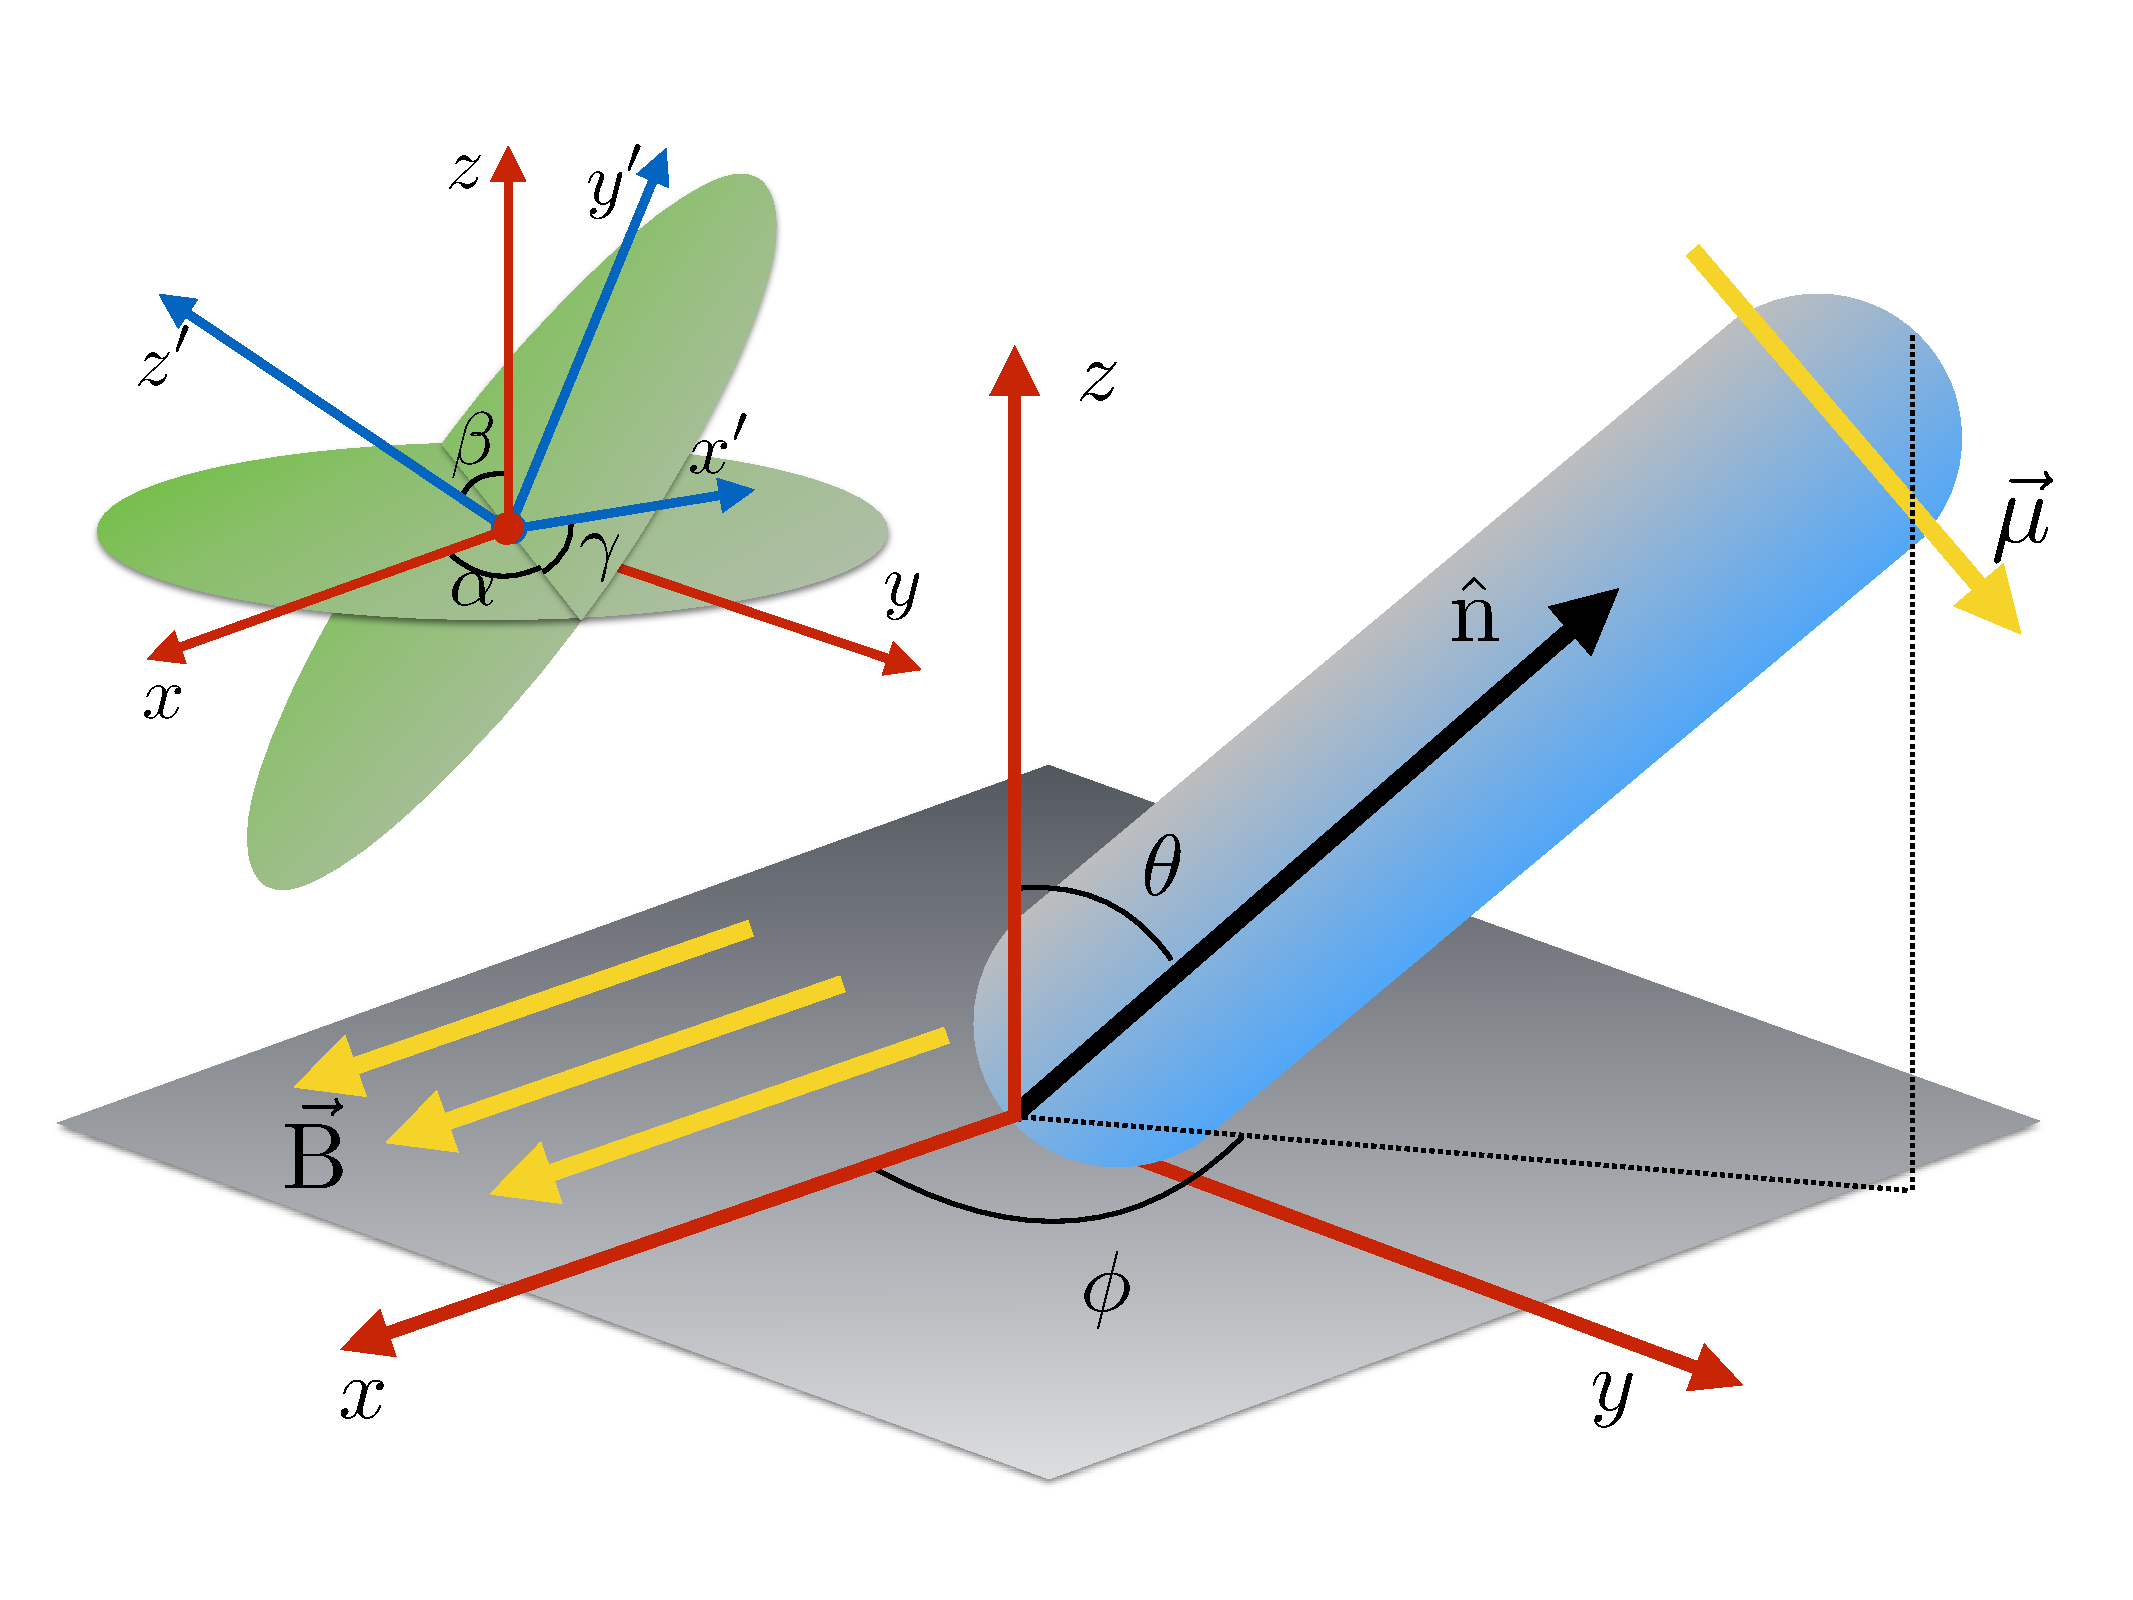
\includegraphics[width=0.98\columnwidth]{figs/geometry.pdf}
	\caption{\footnotesize \emph{Main:} Geometry and notation used throughout. The orientation of the rod, $\hvcrm{n}$ is defined as the unit vector pointing along the long axis of the rod in the $+$ve $z$-direction. This makes an angle $\theta$ with the $z$-axis and its projection in the $xy$-plane subtends an angle $\phi$ with the $x$-axis. A perpendicular permanent magnetic moment $\vc{\mu}$ is embedded in one of the caps and rotates rigidly with the rod. An external magnetic field $\vcrm{B}$ is applied in the $x$-direction while the gravitational field acts in the $-$ve $z$-direction. \emph{Inset:} Euler angles are useful for describing the fixed-body rotation of the rod, where $\hvcrm{n}=\hvcrm{z}'$, $\vc{\mu}=\mu\hvcrm{x}'$, $\beta=\theta$, and $\alpha=\phi+\frac{\pi}{2}$.\label{fig:geometry}}
\end{figure}

\begin{figure}
	\begin{subfigure}[b]{0.48\columnwidth}
    	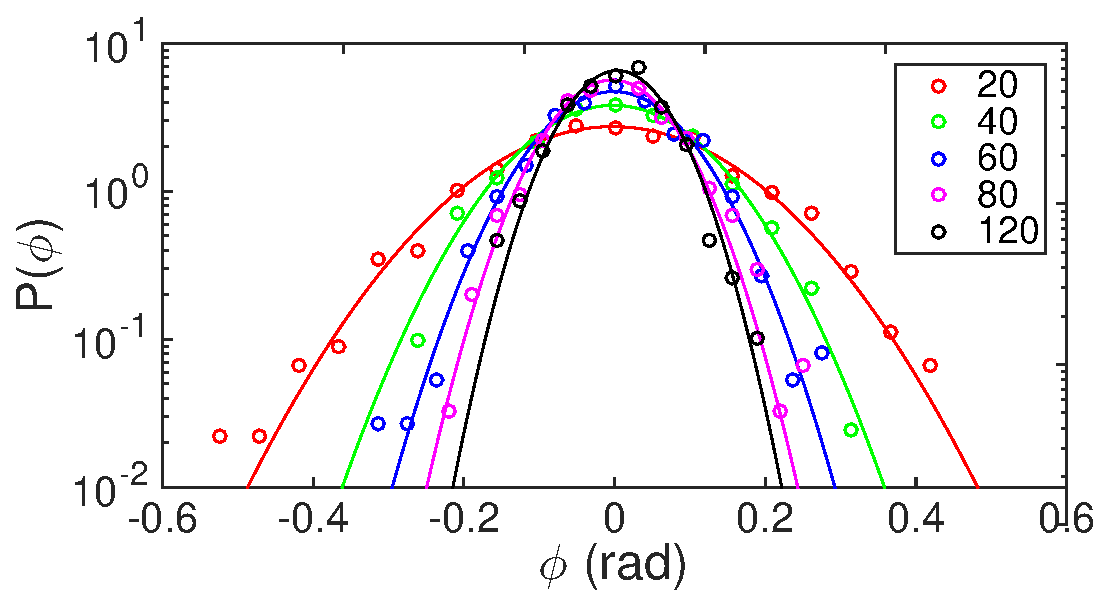
\includegraphics[width=\textwidth]{figs/Figure2a.eps}
    	\caption{}
    \end{subfigure}
    \begin{subfigure}[b]{0.48\columnwidth}
    	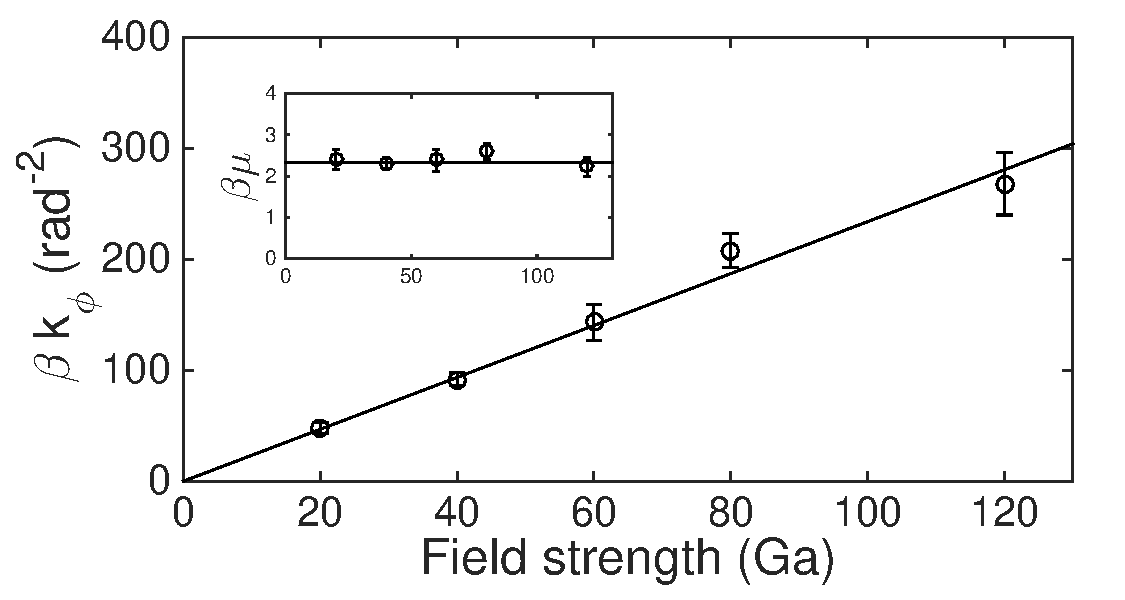
\includegraphics[width=\textwidth]{figs/Figure2b.eps}
    	\caption{}
    \end{subfigure}
    \caption{\footnotesize (a) Probability distribution of the azimuthal angle of deviation $\phi-\phi_0$ of the rod from alignment with a static magnetic field. The data appear to be distributed normally with a spread $\langle \phi^2 \rangle$ obtained by applying a Gaussian fit. (b) The equipartition theorem states $\frac{1}{2} k_\phi \langle \phi^2 \rangle = \frac{1}{2}\kk T$ where $k_\phi =\mu B$ is the stiffness of the torsional trap. We make use of this to show that $\kk T / \langle \phi^2 \rangle $ increases linearly with $B$, in other words, $\mu$ remains constant (see inset) across the range of field strengths used.\label{fig:trap}}
	\label{fig:moment}
\end{figure}




\begin{figure}
\begin{subfigure}[t]{0.26\columnwidth}
    	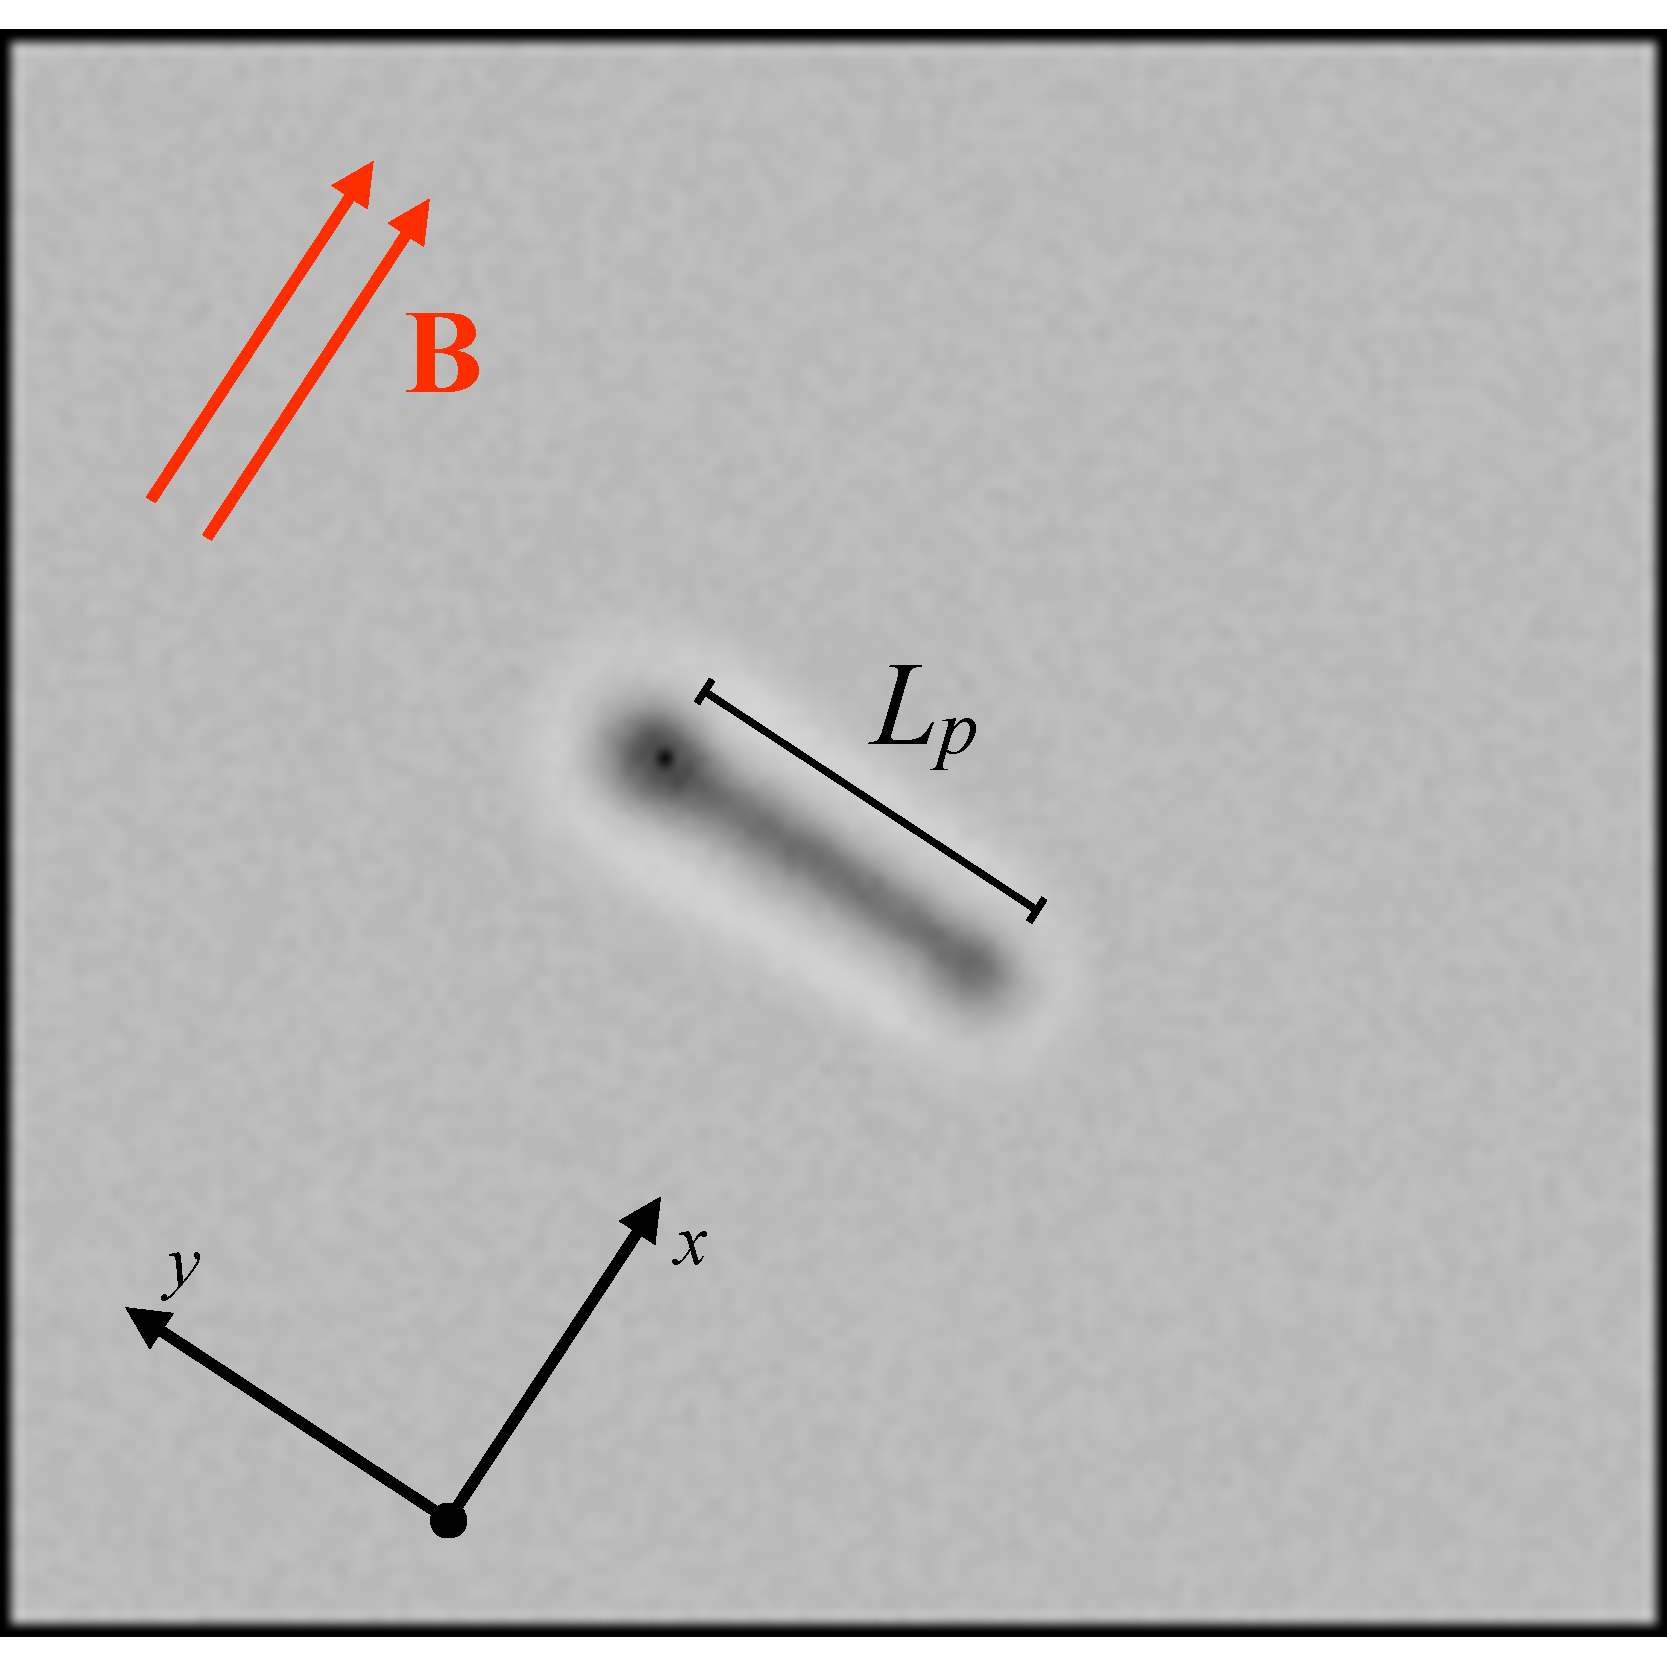
\includegraphics[width=\textwidth]{figs/Figure3bb}
    	\caption{\label{horizontal}}
    \end{subfigure}
	\begin{subfigure}[t]{0.26\columnwidth}
    	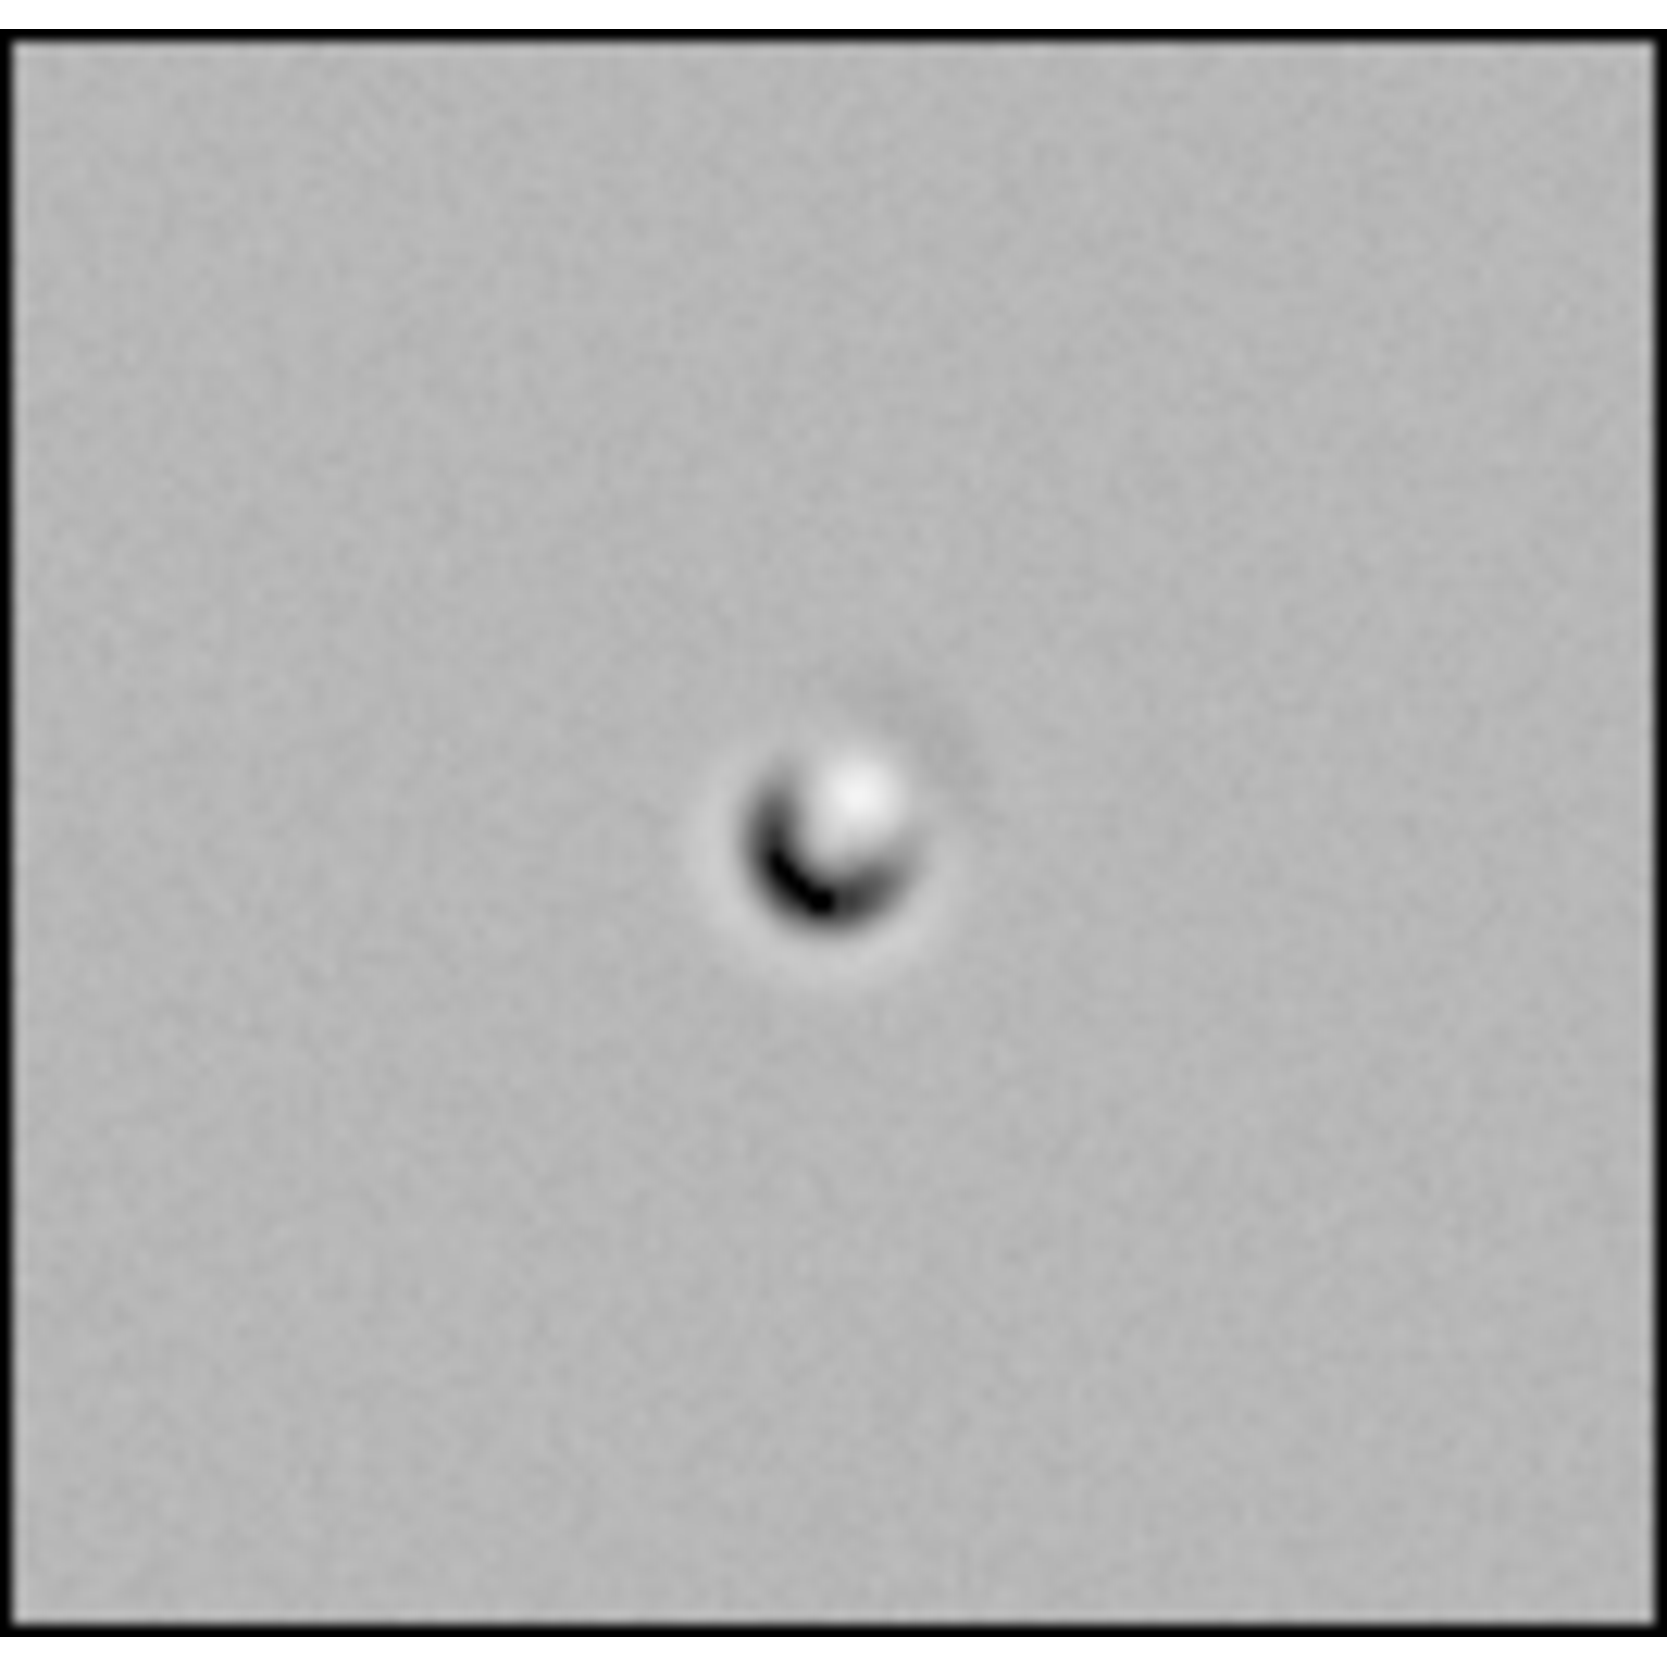
\includegraphics[width=\textwidth]{figs/Figure3ba}
    	\caption{\label{vertical}}
    \end{subfigure}
    \begin{subfigure}[t]{0.26\columnwidth}
    	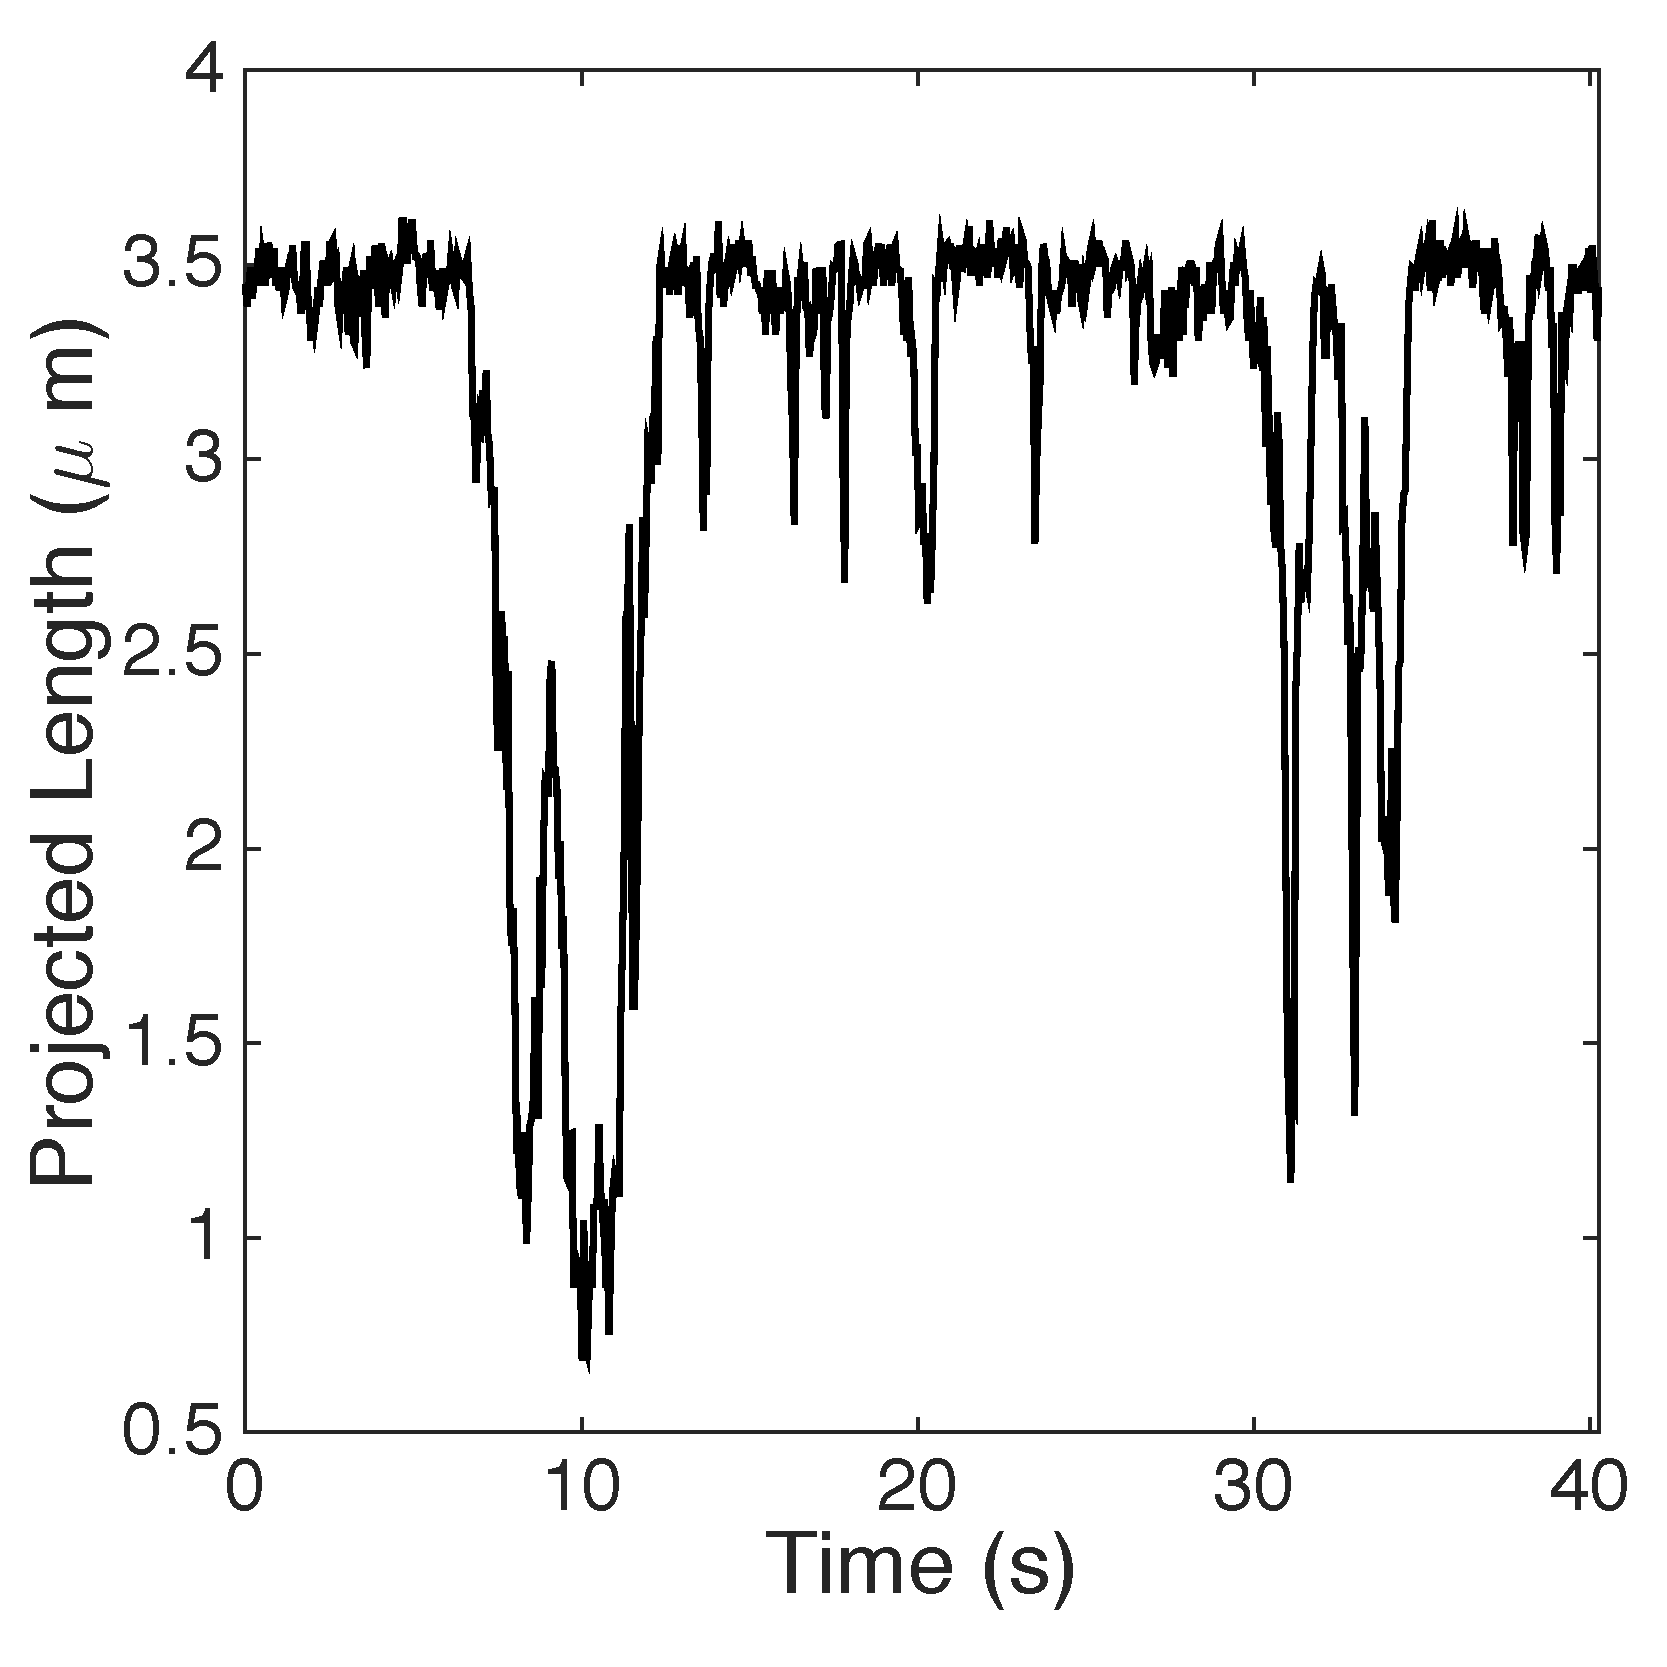
\includegraphics[width=\textwidth]{figs/Figure3bc}
    	\caption{\label{timeseries}}
    \end{subfigure}
    \begin{subfigure}[b]{0.44\columnwidth}
    	\includegraphics[width=\textwidth]{figs/Phi_vs_L_0G.eps}
    	\caption{$B = 0$ Ga \label{Pxy_data}}
    \end{subfigure}
    \begin{subfigure}[b]{0.44\columnwidth}
    	\includegraphics[width=\textwidth]{figs/Phi_vs_L_140G.eps}
    	\caption{$B = 140$ Ga \label{Pxy_data2}}
    \end{subfigure}
    \begin{subfigure}[b]{0.88\columnwidth}
    	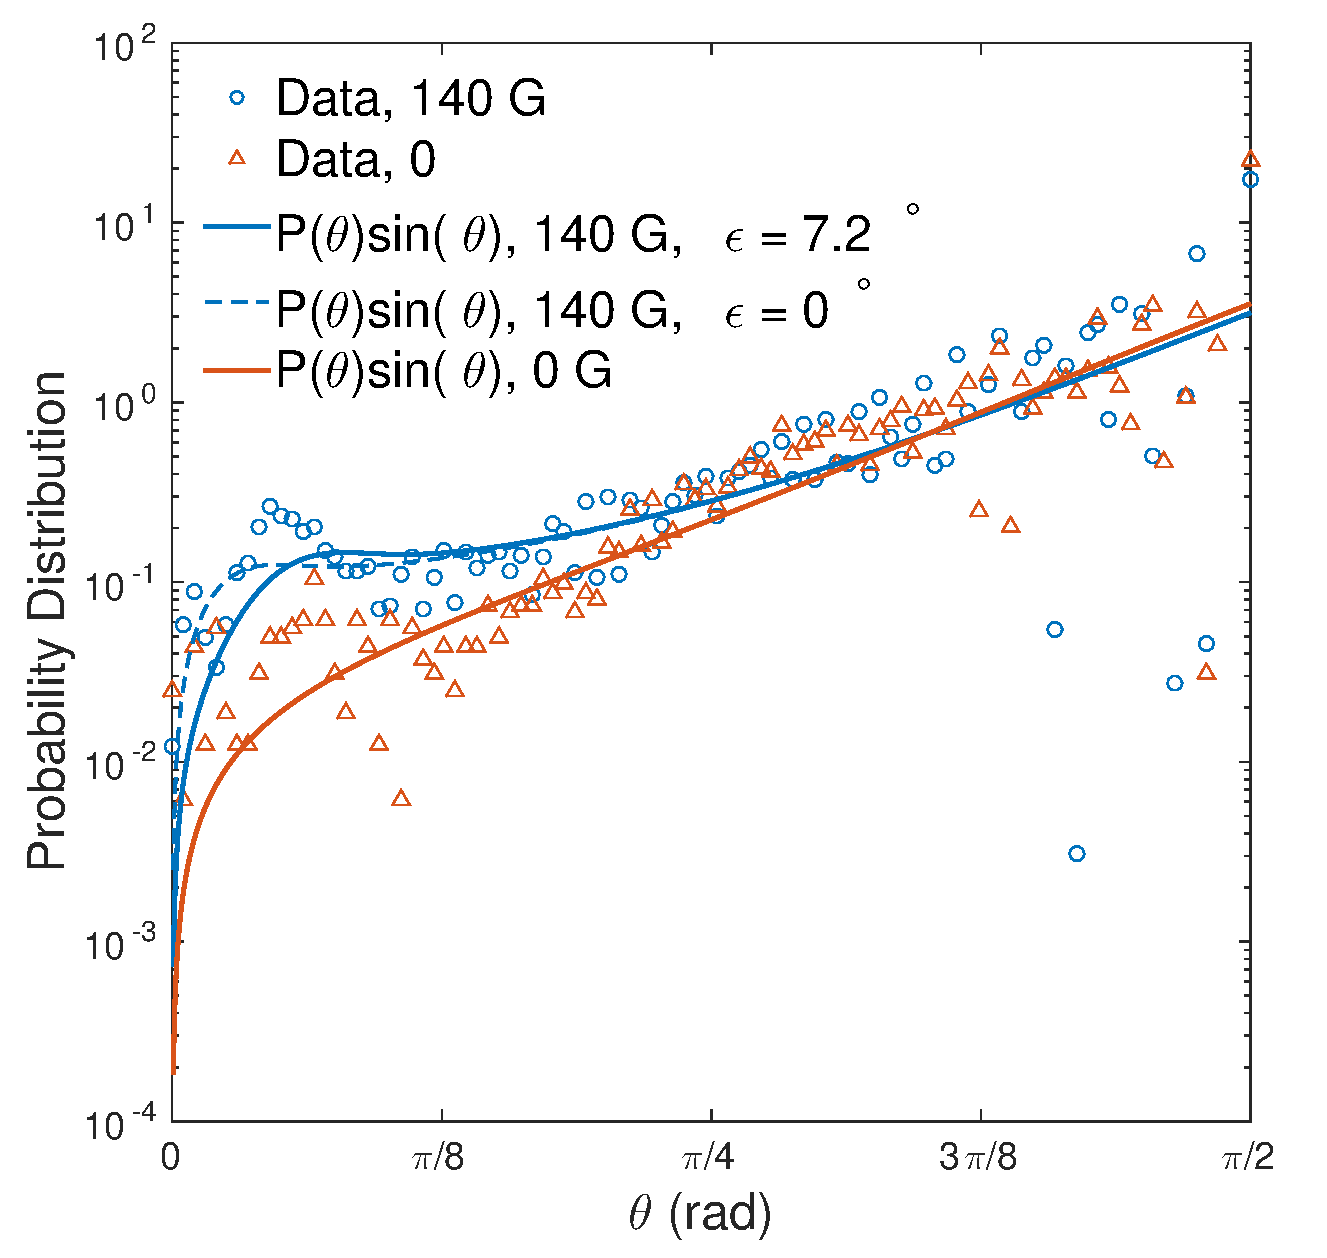
\includegraphics[width=\textwidth]{figs/Figure3a.eps}
    	\caption{\label{Pdata}}
    \end{subfigure}
    \caption{\footnotesize (a-b) A magnetic field in the $x$-direction is responsible for the trapping of the rod in the $yz$-plane; we observe the rod to hop between two states: (a) horizontally along $\pm x$ with $\theta=\pi/2$, and (b) vertically along $z$, where $\theta=0$. (c) A short segment of projected length $L_p(t)$ demonstrates the `hopping' nature of this behaviour. (d-e) The distributions of $\theta(t)$-$\phi(t)$ data falls on top of the theoretically predicted distributions $P(\phi,\theta)|_{B=0,140\ \text{Ga}}$. The trapping angle of the rod $|\phi_0|=(82.8\pm0.2)^\circ < \pi/2$ suggests that the magnetic moment is not quite perpendicular to the rod, making an angle $\epsilon=(7.2\pm0.2)^\circ$ with cross-sectional plane. The radial pattern in the data is an artefact of propagating the measured projected length, $L_p$, through an inverse sine function in the calculation of $\theta$ (f) Histogram of $L_p(t)$ over 60 minutes shows a markedly increased tendency for vertical states ($L_p \approx 1 \mu$m) to be realised when a magnetic field is present (blue) with respect to a free rod, under no magnetic field (red).}
\end{figure}

\begin{figure}
\begin{subfigure}[t]{0.45\columnwidth}
    	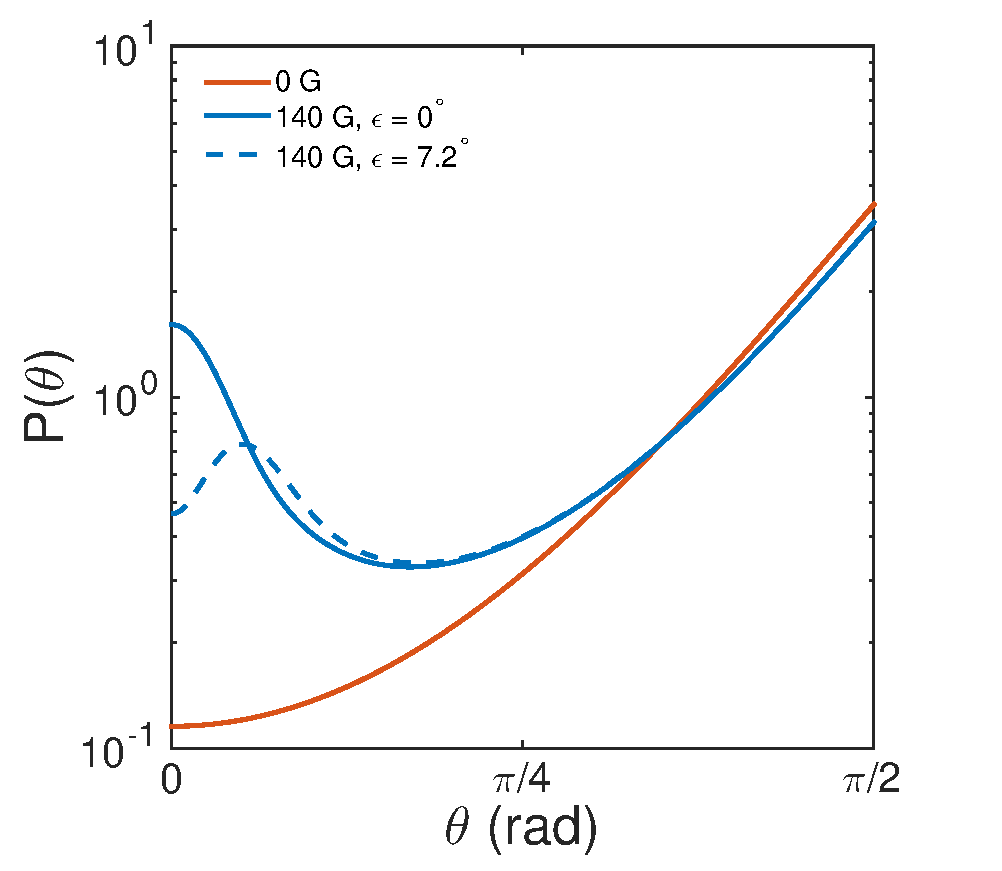
\includegraphics[width=\textwidth]{figs/Figure4.eps}
    	\caption{\label{theorya}}
    \end{subfigure}
	\begin{subfigure}[t]{0.45\columnwidth}
    	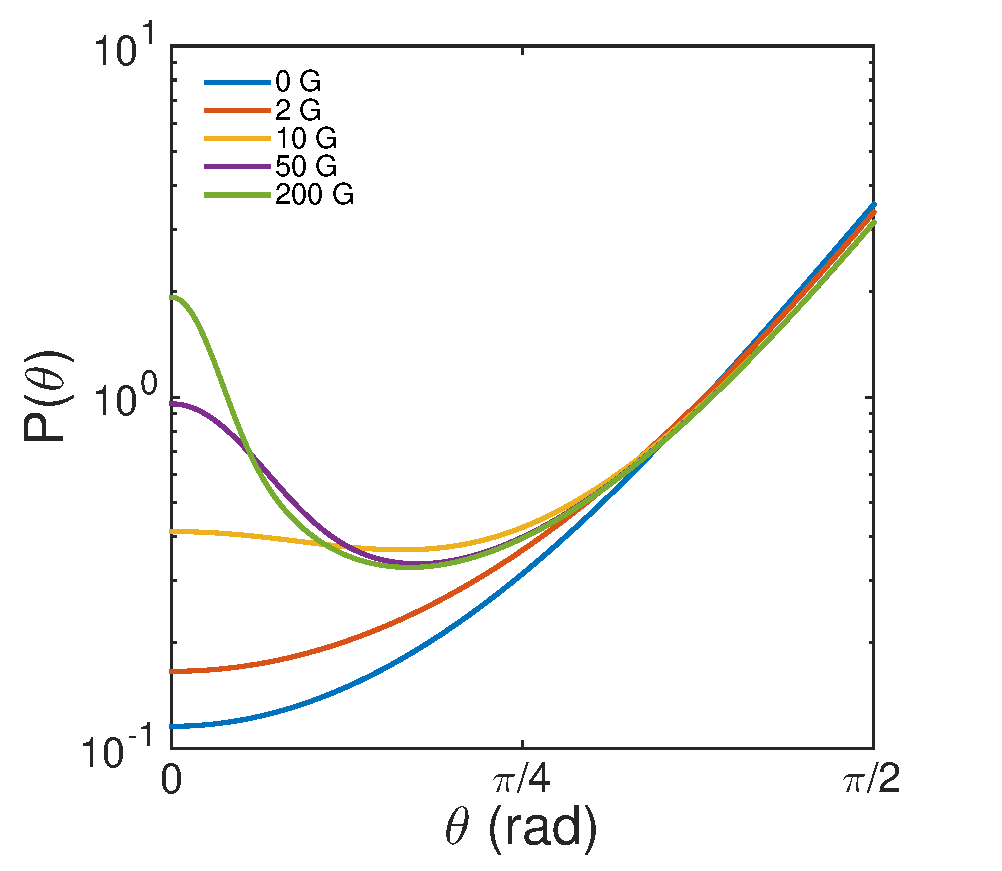
\includegraphics[width=\textwidth]{figs/Figure4b.eps}
    	\caption{\label{theoryb}}
    \end{subfigure}
    \begin{subfigure}[t]{0.32\columnwidth}
    	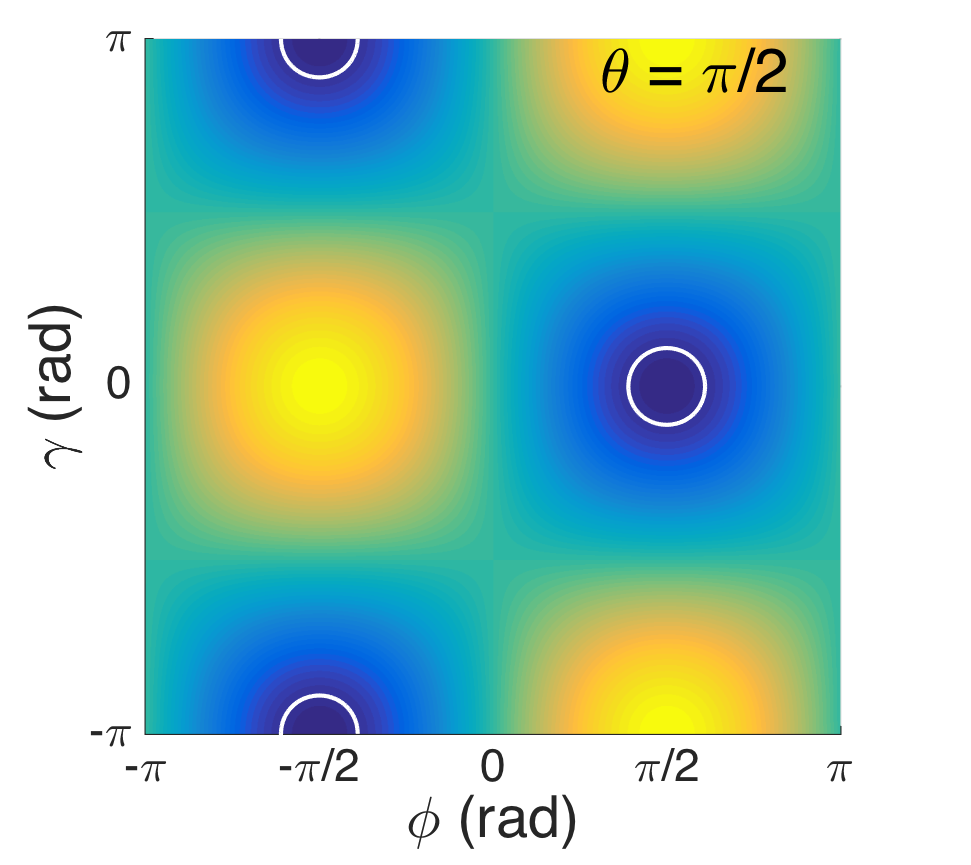
\includegraphics[width=\textwidth]{figs/Figure5a.eps}
    	\caption{\label{phasea}}
    \end{subfigure}
    \begin{subfigure}[t]{0.32\columnwidth}
    	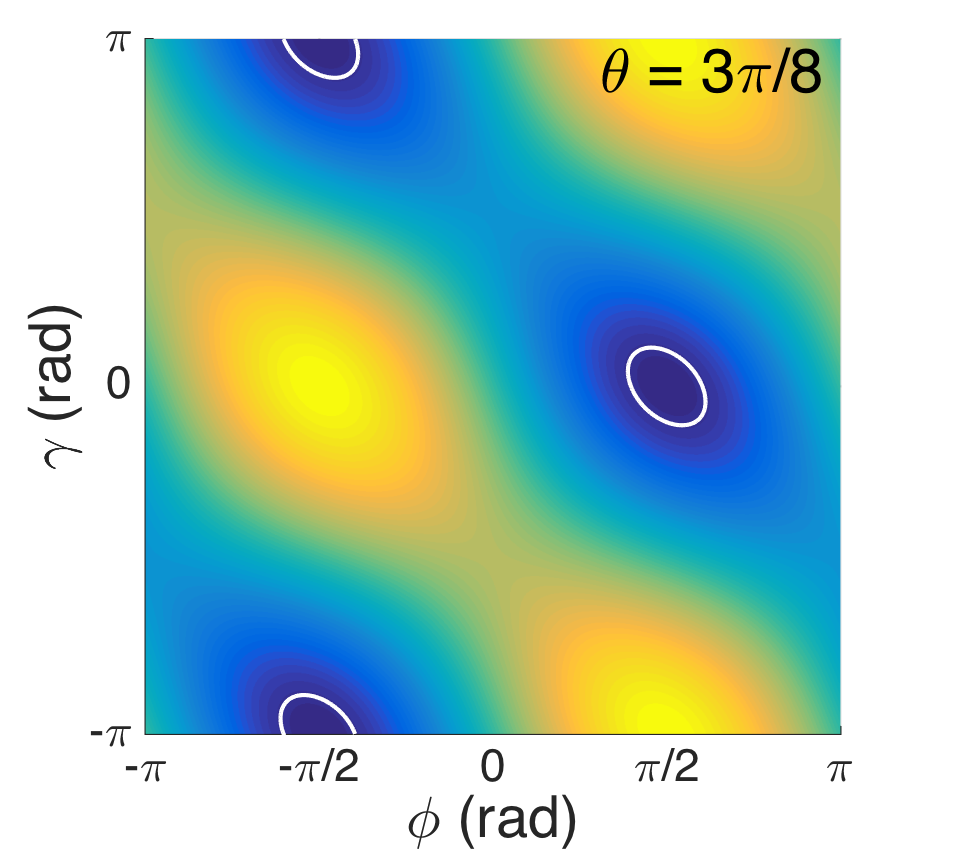
\includegraphics[width=\textwidth]{figs/Figure5b.eps}
    	\caption{\label{phaseb}}
    \end{subfigure}
    \begin{subfigure}[t]{0.32\columnwidth}
    	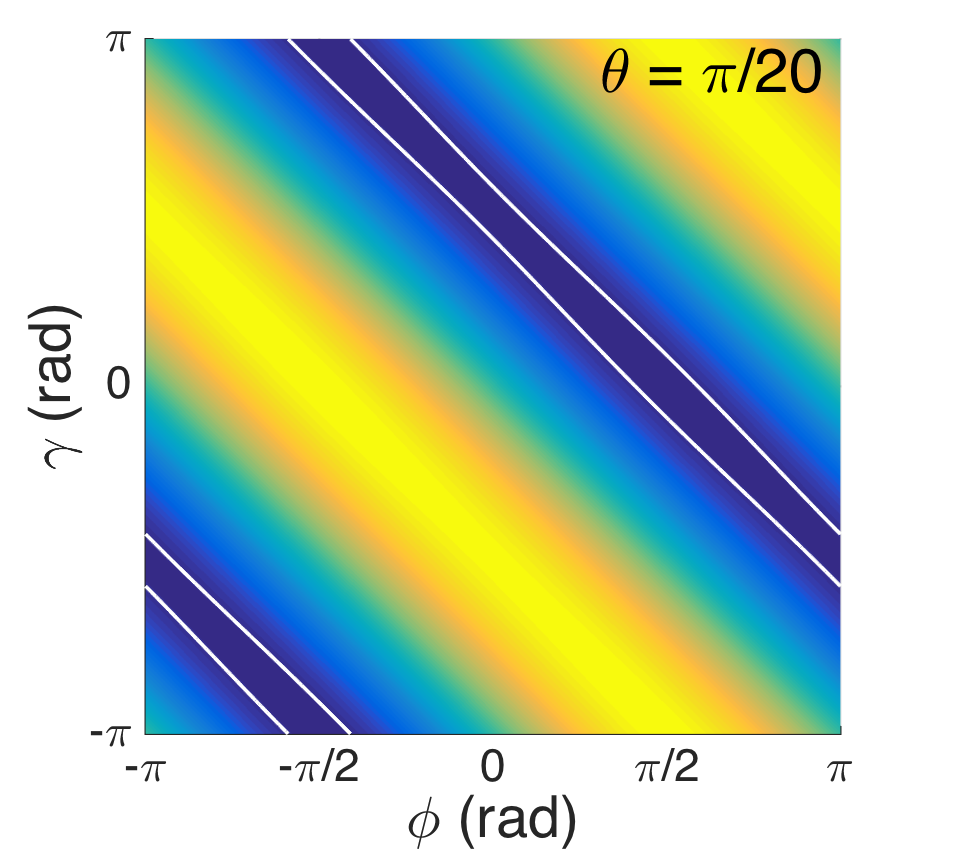
\includegraphics[width=\textwidth]{figs/Figure5c.eps}
    	\caption{\label{phasec}}
    \end{subfigure}
    \caption{\footnotesize (a) Probability distribution for a rod with $\mu=1.2 \kk T/Ga$ in $140$ Ga (blue) and $0$ Ga (red) fields shows an emergent bistability between vertical and horizontal states brought on by the external field for an ideal rod (---) and one where $\vc{\mu}$ is offset from the cross-sectional plane by $\epsilon=7^\circ$ (- -). Inset: Relative likelihood ratio between both probability distributions. (b) Same as (a) but for varying magnetic fields. (c-e) The energy $U(\phi,\theta,\gamma)$ for three polar angles $\theta=\frac{\pi}{2},\frac{3\pi}{8},\frac{\pi}{20}$ shows the loss of a degree of freedom. When the rod is lying flat, $\phi$ and $\gamma$ are independently constrained, but when vertical only the sum $\phi+\gamma$ is constrained. This results in the entropic favouring of vertical states compared to intermediate states despite the gravitational cost of standing up. \label{theory}}
\end{figure}


%For a rod pivoting about one of its ends, it feels a gravitational torque $\vc{\tau}_g = \frac{m^* L}{2} \hvcrm{n}\times\vcrm{g}$, where $\vcrm{g} = -g\hvcrm{z}$ is the gravitational acceleration. In the presence of an external magnetic field, an additional torque $\vc{\tau}_B = \hvc{\mu}\times\vcrm{B}$ is felt. At $T=290$ K, the characteristic strengths of these torques are $|\vc{\tau}_g| \sim 6 \kk$T, and $|\vc{\tau}_B| \sim\ $0-250$\ \kk$T (for fields in the range of $B=\ $0-120 Ga)

%\emph{Distribution}


%\section{}
% Put \label in argument of \section for cross-referencing
%\section{\label{}}
%\subsection{}
%\subsubsection{}

% If in two-column mode, this environment will change to single-column
% format so that long equations can be displayed. Use
% sparingly.
%\begin{widetext}
% put long equation here
%\end{widetext}

% figures should be put into the text as floats.
% Use the graphics or graphicx packages (distributed with LaTeX2e)
% and the \includegraphics macro defined in those packages.
% See the LaTeX Graphics Companion by Michel Goosens, Sebastian Rahtz,
% and Frank Mittelbach for instance.
%
% Here is an example of the general form of a figure:
% Fill in the caption in the braces of the \caption{} command. Put the label
% that you will use with \ref{} command in the braces of the \label{} command.
% Use the figure* environment if the figure should span across the
% entire page. There is no need to do explicit centering.

% \begin{figure}
% \includegraphics{}%
% \caption{\label{}}
% \end{figure}

% Surround figure environment with turnpage environment for landscape
% figure
% \begin{turnpage}
% \begin{figure}
% \includegraphics{}%
% \caption{\label{}}
% \end{figure}
% \end{turnpage}

% tables should appear as floats within the text
%
% Here is an example of the general form of a table:
% Fill in the caption in the braces of the \caption{} command. Put the label
% that you will use with \ref{} command in the braces of the \label{} command.
% Insert the column specifiers (l, r, c, d, etc.) in the empty braces of the
% \begin{tabular}{} command.
% The ruledtabular enviroment adds doubled rules to table and sets a
% reasonable default table settings.
% Use the table* environment to get a full-width table in two-column
% Add \usepackage{longtable} and the longtable (or longtable*}
% environment for nicely formatted long tables. Or use the the [H]
% placement option to break a long table (with less control than 
% in longtable).
% \begin{table}%[H] add [H] placement to break table across pages
% \caption{\label{}}
% \begin{ruledtabular}
% \begin{tabular}{}
% Lines of table here ending with \\
% \end{tabular}
% \end{ruledtabular}
% \end{table}

% Surround table environment with turnpage environment for landscape
% table
% \begin{turnpage}
% \begin{table}
% \caption{\label{}}
% \begin{ruledtabular}
% \begin{tabular}{}
% \end{tabular}
% \end{ruledtabular}
% \end{table}
% \end{turnpage}

% Specify following sections are appendices. Use \appendix* if there
% only one appendix.
%\appendix
%\section{}

% If you have acknowledgments, this puts in the proper section head.
%\begin{acknowledgments}
% put your acknowledgments here.
%\end{acknowledgments}

% Create the reference section using BibTeX:
\bibliography{refs/refs.bib}

\end{document}
%
% ****** End of file apstemplate.tex ******

